\documentclass[professionalfonts,compress,unicode]{beamer}

\usepackage{amsmath,amssymb}
\usepackage{empheq}
\usepackage[utf8]{inputenc}

\usepackage[russian]{babel}

\usepackage{ifthen}

\def\[#1\]{\begin{align*}#1\end{align*}}

\newcommand\myframe[3][dup]{
\ifthenelse{\equal{#1}{}}{}{\ifthenelse{\equal{#1}{dup}}{\subsection{#2}}{\subsection{#1}}}
\frame{\frametitle{#2}{#3}}%
}

\usetheme{Warsaw}
\usecolortheme{uranix}

\setbeamertemplate{headline}
{%
  \begin{beamercolorbox}[sep=0.3cm,wd=\paperwidth]{section in head/foot}%
    \usebeamerfont{frametitle}%
    \vbox{}\vskip-1ex%
    \strut\insertsectionhead\strut\par%
    \vskip-1ex%
  \end{beamercolorbox}%
}
\setbeamertemplate{navigation symbols}{}
\setbeamertemplate{footline}{}
\setbeamertemplate{caption}[numbered]

\renewcommand{\thefootnote}{\fnsymbol{footnote}}

\graphicspath{{images//}}

\title[Волновое уравнение]{Волновое уравнение}
\author[Цыбулин И.В.]{Скалько Юрий Иванович\\
\textbf{Цыбулин Иван}
\\Шевченко Александр}
\date{}
%\vspace{0.3cm}

\begin{document}

{
\setbeamertemplate{headline}[default]
\frame{\titlepage}
}

\section{Волновое уравнение}

\myframe{Волновое уравнение второго порядка}
{
	Волновое уравнение в форме уравнения второго порядка записаывается как
	\[
	\frac{\partial^2 u}{\partial t^2} = c^2\frac{\partial^2 u}{\partial x^2} + f
	\]
	Дополним уравнение до начально-краевой задачи
	\[
	&\left. u\right|_{t=0} = \varphi(x)\\
	&\left. \frac{\partial u}{\partial t}\right|_{t=0} = \theta(x)\\
	&\left. \frac{\partial u}{\partial x}\right|_{x=0} = \psi(t)\\
	&\left. u\right|_{x=1} = \chi(t)
	\]
}

\myframe{Схема <<крест>>}
{
	\begin{columns}[T]
	\begin{column}{0.8\textwidth}%
	Аппроксимация на шаблоне крест получается при замене 
	вторых производных их разностными аналогами. Порядок аппроксимации уравнения второй 
	по пространству и времени.	
	\end{column}%
	\begin{column}{0.2\textwidth}%
	\begin{figure}%
	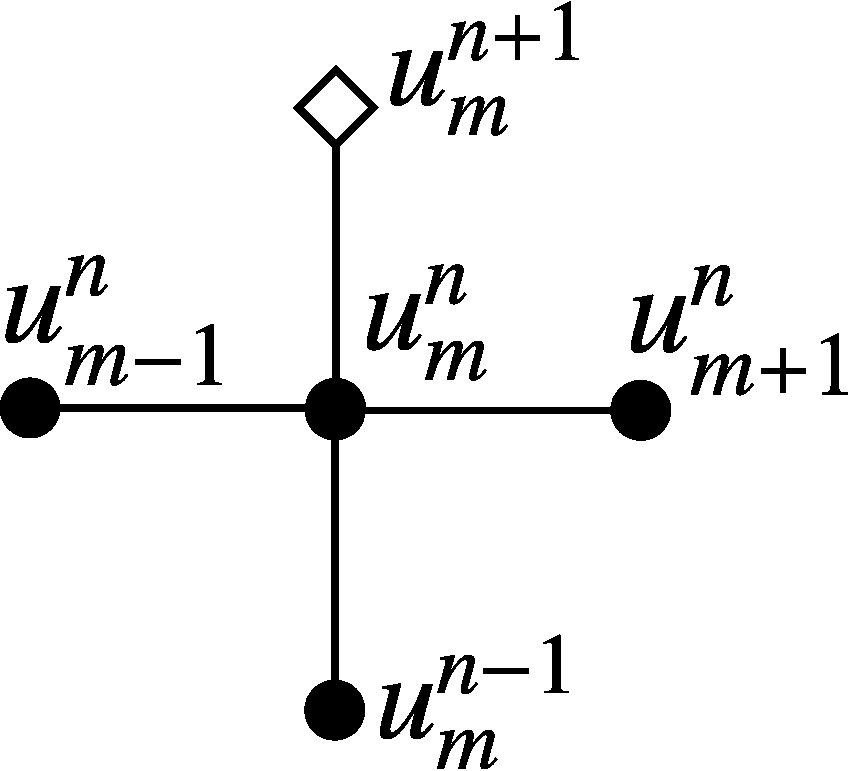
\includegraphics[width=\columnwidth]{cross.pdf}%
	\end{figure}
	\end{column}
	\end{columns}
	\[
	\frac{u^{n+1}_m-2u^{n}_m+u^{n-1}_m}{\tau^2} = c^2\frac{u^n_{m+1}-2u^n_m+u^n_{m-1}}{h^2} + f^n_m
	\]
	Простейшая аппроксимация граничных и начальных условий
	\[
	u^0_m &= \varphi_m + O(\tau^\infty+h^\infty)\\
	\frac{u^1_m-u^0_m}{\tau} &= \theta_m + O(\tau+h^\infty)\\
	\frac{u^n_1-u^n_0}{h} &= \psi^n + O(\tau^\infty+h)\\
	u^n_M &= \chi^n + O(\tau^\infty+h^\infty)
	\]
}

\myframe{Повышение порядка начальных условий}
{
	Вынесем из $O(\cdot)$ члены первого порядка
	\[
	\frac{u^1_m-u^0_m}{\tau} &= \theta_m + \frac{\tau}{2}[u_{tt}]^0_m + O(\tau^2+h^\infty)
	\]
	Необходимо аппроксимировать $u_{tt}$ хотя бы с первым порядком по $\tau$ в точке $(t_0,x_m)$.
	Например, можно подставить 
	\[[u_{tt}]^0_m = c^2[\varphi'']_m+f^0_m+ O(\tau^\infty+h^\infty)\] 
	(уравнение при $t=0$) если $\varphi(x)$ задана
	аналитически или
	\[[u_{tt}]^0_m = c^2\frac{\varphi_{m+1}-2\varphi_{m}+\varphi_{m-1}}{h^2}+f^0_m+ O(\tau^\infty+h^2)\]
	если производную вычислить сложно. В результате
	\[
	\frac{u^1_m-u^0_m}{\tau} &= \theta_m + \frac{\tau}{2}\left\{c^2\frac{\varphi_{m+1}-2\varphi_{m}+\varphi_{m-1}}{h^2}+f^0_m\right\} + O(\tau^2+\tau h^2)
	\]
}

\myframe{Повышение порядка грачничных условий}
{
	Вынесем из $O(\cdot)$ члены первого порядка
	\[
	\frac{u^n_1-u^n_0}{h} &= \psi^n + \frac{h}{2}[u_{xx}]^n_0 + O(\tau^\infty+h^2)
	\]
	Необходимо аппроксимировать $u_{xx}$ хотя бы с первым порядком по $h$ в точке $(t_n,0)$.
	Например, можно подставить 
	\[[u_{xx}]^n_0 = \frac{u^n_2 - 2u^n_1 + u^n_0}{h^2} + O(h + \tau^\infty)\] 
	(в крайних точках формула первого порядка). В результате
	\[
	\frac{u^n_1-u^n_0}{h} &= \psi^n +\frac{u^n_2 - 2u^n_1 + u^n_0}{2h} + O(\tau^\infty+h^2)
	\]
	Это уравнение легко разрешается относительно $u^n_0$. Необходимые значения $u^n_1$ и $u^n_2$ уже должны быть
	посчитаны по схеме <<крест>> из временных слоев $n-1$ и $n-2$.
}

\myframe{Устойчивость схемы <<крест>>} 
{
	Исследуем схему <<крест>> на устойчивость по спектральному признаку. Подставим $u^n_m = \lambda^n e^{i \alpha m}$
	\[
	&\frac{\lambda - 2 + \frac{1}{\lambda}}{\tau^2} = \frac{e^{i\alpha}-2+e^{-i\alpha}}{h^2} = -\frac{4}{h^2}\sin^2 \frac{\alpha}{2}\\
	&\lambda^2 - 2\left(1 - \frac{2\tau^2}{h^2}\sin^2 \frac{\alpha}{2}\right)\lambda + 1 = 0\\
	&\lambda_1 \lambda_2 = 1\\
	&\frac{D}{4} = \left(\frac{2\tau^2}{h^2}\sin^2 \frac{\alpha}{2} - 1\right)^2 - 1 = 
	\frac{2\tau^2}{h^2}\sin^2 \frac{\alpha}{2}\left(\frac{2\tau^2}{h^2}\sin^2 \frac{\alpha}{2} - 2\right)
	\]
	При $D>0$ корни действительные и хотя бы одно из чисел $|\lambda_1|, |\lambda_2|$ больше единицы. При отрицательном 
	$D$ корни комплексно сопряжены и оба по модулю равны $1$. Схема устойчива при $D<0$, то есть при $\tau < h$
}

\myframe{Волновое уравнение в виде системы первого порядка}
{
	Введем $v = u_t, w = u_x$. В этих обозначениях волновое уравнение можно записать как систему
	\[
	\frac{\partial}{\partial t}\begin{pmatrix}
		v \\ w
	\end{pmatrix} +
	\begin{pmatrix}
		0 & -c^2\\
		-1 & 0
	\end{pmatrix}
	\frac{\partial}{\partial x}\begin{pmatrix}
		v \\ w
	\end{pmatrix}	=
	\begin{pmatrix}
		f \\ 0
	\end{pmatrix}
	\]
	Найдем левые собственные вектора ${\boldsymbol\omega}_i^T \mathbf{A} = \lambda_i {\boldsymbol\omega}_i^T$ (собственные вектора транспонированной матрицы)
	\[
	\begin{pmatrix}
	1&c
	\end{pmatrix}
	\begin{pmatrix}
		0 & -c^2\\
		-1 & 0
	\end{pmatrix}
	=-c
	\begin{pmatrix}
	1&c
	\end{pmatrix}\quad 
	{\boldsymbol\omega}_1 = \begin{pmatrix}
	1\\c	
	\end{pmatrix}\quad \lambda_1 = -c
	\\
	\begin{pmatrix}
	1&-c
	\end{pmatrix}	
	\begin{pmatrix}
		0 & -c^2\\
		-1 & 0
	\end{pmatrix}
	=c
	\begin{pmatrix}
	1&-c
	\end{pmatrix}\quad 
	{\boldsymbol\omega}_2 = \begin{pmatrix}
	1\\-c
	\end{pmatrix}\quad \lambda_2 = c
	\]
	Умножим систему слева на ${\boldsymbol\omega}_i^T$
}

\myframe{Система в инвариантах}
{
При умножении на левые собственные вектора система распадается на отдельные уравнения переноса
\[
	\frac{\partial(v+cw)}{\partial t} - c \frac{\partial(v+cw)}{\partial x} = f\\
	\frac{\partial(v-cw)}{\partial t} + c \frac{\partial(v-cw)}{\partial x} = f
\]
Любая система гиперболического типа 
\[
\frac{\partial \mathbf{u}}{\partial t} + \mathbf{A} \frac{\partial \mathbf{u}}{\partial x} = \mathbf{f}
\]
при умножении на левый собственный вектор ${\boldsymbol\omega}_i^T \mathbf{A} = \lambda_i {\boldsymbol\omega}_i^T$ распадается на уравнения переноса
\[
\frac{\partial({\boldsymbol\omega}_i,\mathbf{u})}{\partial t} + \lambda_i \frac{\partial({\boldsymbol\omega}_i,\mathbf{u})}{\partial x} = ({\boldsymbol\omega}_i,\mathbf{f})
\]
Скалярные величины $r_i = ({\boldsymbol\omega}_i,\mathbf{u})$ называются \emph{инвариантами Римана}
}

\myframe{Схема для уравнения}
{
	Поскольку система уравнений распалась на независимые уравнения переноса, напишем для каждого уравнения переноса схему явный левый или явный правый уголок,
	в зависимости от $\lambda_i > 0$ или $\lambda_i < 0$. 
	\[
	&\frac{(r_i)^{n+1}_m-(r_i)^n_m}{\tau} + \lambda_i \frac{(r_i)^n_m-(r_i)^n_{m-1}}{h} = ({\boldsymbol\omega}_i,\mathbf{f})^n_m, \; m = \overline{1,M}, \; \lambda_i > 0\\
	&\frac{(r_i)^{n+1}_m-(r_i)^n_m}{\tau} + \lambda_i \frac{(r_i)^n_{m+1}-(r_i)^n_m}{h} = ({\boldsymbol\omega}_i,\mathbf{f})^n_m, \; m = \overline{0,M-1}, \lambda_i < 0
	\]
	Если $\lambda_i = 0$, то уравнение переноса вырождается в обыкновенное дифференциальное уравнение
	\[
	\frac{\partial r_i}{\partial t} = ({\boldsymbol\omega}_i,\mathbf{f}),
	\]
	которое решается при всех значениях $m$
	\[
	\frac{(r_i)^{n+1}_m-(r_i)^n_m}{\tau} = ({\boldsymbol\omega}_i,\mathbf{f})^n_m, \quad m = \overline{0,M}
	\]
}

\myframe{Граничные условия}
{
	Для численного решения системы необходимы начальные и граничные условия. Поскольку уравнения аппроксимированы с первым порядком (уголками), то достаточно потребовать
	первого порядка аппроксимации граничных условий.
	
	Рассмотрим сколько необходимо граничных условий для волнового уравнения. Запишем схемы для инвариантов
	\[
	&\frac{(r_1)^{n+1}_m-(r_1)^n_m}{\tau} - c \frac{(r_1)^n_{m+1}-(r_1)^n_m}{h} = f^n_m, \quad m = \overline{0,M-1}\\
	&\frac{(r_2)^{n+1}_m-(r_2)^n_m}{\tau} + c \frac{(r_2)^n_m-(r_2)^n_{m-1}}{h} = f^n_m, \quad m = \overline{1,M}
	\]
	По этим схемам нельзя определить $r_1$ при $m=M$ и $r_2$ при $m=0$. Эти значения необходимо найти из граничных условий. Значит, необходимо по одному 
	граничному условию на каждой границе.
}

\myframe{Схема для граничных узлов}
{
	Зададим, для примера, следующие граничные условия (по 1му на каждой границе)
	\[
	v|_{x=0} = 0\\
	(v-cw)|_{x=1} = 1
	\]
	Попробуем с помощью них найти $(r_1)^n_M$ и $(r_2)^n_0$ при известных остальных значениях на слое $n$. Для этого выразим исходные
	неизвестные через инварианты
	\[
	v = \frac{r_1+r_2}{2}\\
	w = \frac{r_1-r_2}{2c}
	\]
	Граничные условия в инвариантах
	\[
	r_1+r_2|_{x=0} = 0\\
	r_2|_{x=1} = 1
	\]	
}

\myframe[]{Схема для граничных узлов}
{
	Граничные условия в инвариантах
	\[
	(r_1+r_2)_0^n = 0\\
	(r_2)_M^n = 1
	\]
	Из уголков для внутренних точек можно найти $(r_1)^n_0$ и $(r_2)^n_M$. $(r_1)^n_M$ и $(r_2)^n_0$ необходимо искать привлекая граничные условия.
	Легко найти $(r_2)^n_0 = (r_1+r_2)_0^n - (r_1)^n_0 = -(r_1)^n_0$. Но $(r_1)^n_M$ из этих данных найти не получится. Более того, значение 
	$(r_2)^n_M$ находится как с помощью схемы для внутренних точек, так и задается граничным условием!
	
	Данная задача является некорректно поставленной.
}

\myframe[]{Корректность условий для гиперболической системы}
{
	Пусть для гиперболической системы с $\Lambda^{-}$ отрицательными, $\Lambda^{+}$ положительными и $\Lambda^0$ нулевыми собственными числами 
	($\Lambda^- + \Lambda^+ + \Lambda^0 = n$) задано $K^-$ граничных условий слева и $K^+$ граничных условий справа.
	\[
	&({\boldsymbol\alpha}_i, \mathbf{u})|_{x=0} = \beta_i, \quad i = \overline{1,K^{-}}\\
	&({\boldsymbol\alpha}_i, \mathbf{u})|_{x=1} = \beta_i, \quad i = \overline{K^{-}+1,K^-+K^+}
	\]
	На левой границе известны значения всех инвариантов для $\lambda_i \leq 0$. Вместе с граничными условиями слева они должны давать невырожденную систему для 
	остальных инвариантов.
}

\myframe[]{Корректность условий для гиперболической системы}
{
	Математически, это выражается в отличии от нуля следующих определителей матриц, составленных из собственных векторов задачи (левых)
	и векторов $\boldsymbol\alpha$ из граничных условий. На левой границе
	\[
	\operatorname{det} \begin{Vmatrix}
	\underbrace{
		{\boldsymbol\omega}_1 \;\dots\;
		{\boldsymbol\omega}_{\Lambda^-} 
		}_{\lambda_i < 0} &
	\underbrace{
		{\boldsymbol\omega}_{\Lambda^-+1} \;	\dots \;
		{\boldsymbol\omega}_{\Lambda^-+\Lambda^0} 
		}_{\lambda_i = 0} &
	\underbrace{	
		{\boldsymbol\alpha}_1 \; \dots \;
		{\boldsymbol\alpha}_{K^{-}}
		}_{x = 0}
	\end{Vmatrix} \neq 0
	\]
	Аналогичные условия должны выполняться на правой границе
	\[
	\operatorname{det} \begin{Vmatrix}
	\underbrace{
		{\boldsymbol\omega}_{\Lambda^-+\Lambda^0+1}  \;\dots\;
		{\boldsymbol\omega}_{n} 
		}_{\lambda_i > 0} &
	\underbrace{
		{\boldsymbol\omega}_{\Lambda^-+1} \;	\dots \;
		{\boldsymbol\omega}_{\Lambda^-+\Lambda^0} 
		}_{\lambda_i = 0} &
	\underbrace{	
		{\boldsymbol\alpha}_{K^-+1} \; \dots \;
		{\boldsymbol\alpha}_{K^-+K^+}
		}_{x = 1}
	\end{Vmatrix} \neq 0
	\]	
}

\myframe{Численная схема в инвариантах}
{
	Численное решение можно искать как в исходных переменных $(u,v)$, так и в инвариантах $(r_1, r_2)$.
	Рассмотрим корректные краевые условия для волнового уравнения $v|_{x=0} = v|_{x=1} = 0$. Численная схема в инвариантах выглядит так:
	\[
	&\frac{(r_1)^{n+1}_m-(r_1)^n_m}{\tau} - c \frac{(r_1)^n_{m+1}-(r_1)^n_m}{h} = f^n_m, \quad m = \overline{0,M-1}\\
	&\frac{(r_2)^{n+1}_m-(r_2)^n_m}{\tau} + c \frac{(r_2)^n_m-(r_2)^n_{m-1}}{h} = f^n_m, \quad m = \overline{1,M}\\
	&(r_1)^{n+1}_M = -(r_2)^{n+1}_M\\
	&(r_2)^{n+1}_0 = -(r_1)^{n+1}_0\\
	&(r_1)^0_m = [v_0-cw_0]_m\\
	&(r_2)^0_m = [v_0+cw_0]_m
	\]
}

\myframe{Алгоритм численного решения задачи}
{
\begin{enumerate}
	\item Значения инвариантов на $0$-м временном слое получаются из начальных условий для $(u,v)$
	\item Пусть слой $n$ уже посчитан. По схемам <<уголок>> рассчитываются инварианты на слое $n+1$, всюду кроме 
	двух граничных узлов. В одном нельзя вычислить инвариант $r_1$, в другом --- $r_2$
	\item Эти значения вычисляются из граничных условий (необходимые для вычислений данные уже найдены)
	\item Слой $n+1$ полностью заполнен, и можно повторять с шага 2
\end{enumerate}
}

\myframe{Численная схема в исходных неизвестных}
{
	Перейдем от инвариантов к исходным переменным
	\[
	&\frac{v^{n+1}_m-v^n_m}{\tau} - c \frac{(v+cw)^n_{m+1}+(v-cw)^n_{m-1}-2v^n_m}{2h} = f^n_m, \; m = \overline{1,M-1}\\
	&\frac{w^{n+1}_m-w^n_m}{\tau} - \frac{(wc+v)^n_{m+1}+(wc-v)^n_{m-1}-2cw^n_m}{2h} = 0, \; m = \overline{1,M-1}\\
	&\frac{(v+cw)^{n+1}_0-(v+cw)^n_0}{\tau} - c \frac{(v+cw)^n_1-(v+cw)^n_0}{h} = f^n_0\\
	&v^{n+1}_0 = 0\\
	&\frac{(v-cw)^{n+1}_M-(v-cw)^n_M}{\tau} + c \frac{(v-cw)^n_M-(v-cw)^n_{M-1}}{h} = f^n_0\\
	&v^{n+1}_M = 0\\
	&v^0_m = [v_0]_m\\
	&w^0_m = [w_0]_m
	\]
}

\myframe{Алгоритм численного решения задачи в исходных переменных}
{
\begin{enumerate}
	\item Значения переменных на $0$-м временном слое получаются из начальных условий
	\item Пусть слой $n$ уже посчитан. По схемам для внутренних точек рассчитываются переменные на слое $n+1$, всюду кроме 
	двух граничных узлов. 
	\item В каждом граничном узле есть два линейных уравнения на две неизвестные $u$ и $v$ в этом узле. Решая системы, получаем
	значение переменных в граничных точках.
	\item Слой $n+1$ полностью заполнен, и можно повторять с шага 2
\end{enumerate}
}

%%%%%%%%%%%%%%%%%%%%%%%%%%%%%%%%%%%%%%%%%%%%%%%
%%%%%%%%%%%%%%%%%%%%%%%%%%%%%%%%%%%%%%%%%%%%%%%
%%%%%%%%%                            %%%%%%%%%%
%%%%%%%%%%%%%%%%%%%%%%%%%%%%%%%%%%%%%%%%%%%%%%%
%%%%%%%%%%%%%%%%%%%%%%%%%%%%%%%%%%%%%%%%%%%%%%%
{
\setbeamertemplate{headline}[default] 
\frame{
	\begin{center}
	{\Huge Спасибо за внимание!}
	\end{center}
	\bigskip
	\begin{center}
	{\color{blue}{tsybulinhome@gmail.com}}
	\end{center}
	}
}

\end{document}